\documentclass[a4paper,twoside]{article}
\usepackage{jmlr2e}
\usepackage{amsmath,amssymb}
%\usepackage[T1]{fontenc}
%\usepackage[latin1]{inputenc}
%\usepackage[dvipdf]{graphicx}
\usepackage{color}
\usepackage[linesnumbered]{algorithm2e}
\usepackage[hidelinks, colorlinks=true, 
linkcolor=black, citecolor=blue]{hyperref} 

\newcommand{\cad}{---} % tiret cadratin
\newcommand{\gl}[1]{``\,#1\,''} % Guillemets standard
\newcommand{\ms}[1]{\texttt{#1}} %racccourci pour ``monospaced''
\newcommand{\lat}{\emph} %pour les mots latins

\newcommand{\ml}[1]{\textcolor{red}{ML : #1}}
\newcommand{\mr}[1]{\textcolor{magenta}{MR : #1}}

\jmlrheading{1}{2000}{1-48}{4/00}{10/00}{Marina Meil\u{a} and Michael I. Jordan}

\begin{document}

\title{the K-averages algorithm \\ a linear optimization alternative to kernel K-means}

\author{Mathias Rossignol \and Mathieu Lagrange}

\editor{}

\maketitle


\begin{abstract}

We present an iterative flat clustering algorithm designed to operate on arbitrary similarity matrices, with the only constraint that these matrices be symmetrical. Although functionally very close to kernel k-means, our proposal performs an maximization of average intra-class similarity, instead of a squared distance minimization, in order to remain closer to the semantics of similarities. We show that this approach allows relaxing the conditions on usable matrices, as well as opening better optimization possibilities. Systematic evaluation on a variety of data sets shows that the proposed approach equals or outperforms kernel k-means in most cases, while running much faster. Most notably, it significantly reduces memory access, which makes it a good choice for very large data collections.

\end{abstract}


\section{Introduction}

Clustering collections of objects into classes that bring together similar ones is probably the most common and intuitive tool used both by human cognition and artificial data analysis in an attempt to make that data organized, understandable, manageable. When the studied objects lend themselves to this kind of analysis, it is a powerful way to expose underlying organizations and approximate the data in such a way that the relationships between its members can be statistically understood and modeled. Given a description of objects, we first attempt to quantify which ones are ``\,similar\,'' from a given point of view, then group those $n$ objects into $C$ clusters, so that the similarity between objects within the same cluster is maximized. Finding the actual best possible partition of objects into clusters is, however, an NP-complete problem, intractable for useful data sizes, and many approaches have been proposed to yield an approximate solution: analytic, iterative, flat or hierarchical, agglomerative or divisive, soft or hard clustering algorithms, \textit{etc.}, each with their strengths and weaknesses (\cite{jain2010data}), performing better on some classes of problems than others (\cite{steinbach2000comparison,thalamuthu2006evaluation}).

Iterative divisive hard clustering algorithms, such as the ubiquitous \emph{k-means}, usually perform well to identify high-level organization in large data collections in reasonable running time; their main drawback being that the number of desired clusters must be specified. For that reason, they are a sensible choice in many data mining situations, and constitute our focus in this paper.

If the data lies in a vector space, \textit{i.e.} an object can be described by a $m$-dimensional feature vector without significant loss of information, the seminal \emph{K-means} algorithm (\cite{macQueenBsmsp67}) is probably the most efficient approach, since the explicit computation of the cluster centroids ensure both computational efficiency and scalability. This algorithm is  based on the centroid model, and minimizes the intra cluster Euclidiean distance. As shown by \cite{Banerjee:2005:CBD:1046920.1194902}, any kind of Bregman divergence, such as the KL-divergence (\cite{Dhillon:2003:DIT:944919.944973}) or the Itakura-Saito divergence (\cite{linde:algorithm}), may also be considered to develop such efficient clustering algorithms.

However, for many types of data, the projection of a representational problem into an vector space cannot be done without significant loss of descriptive efficiency. To reduce this loss, specifically tailored measures of similarity can be considered. As a result, the input data for clustering is no longer a $n \times m$ matrix storing the $m$-dimensional vectors describing the objects, but a (usually symmetric) square matrix $S$ of size $n \times n$ which numerically encodes some sort of relationship between the objects. In this case, one has to resort to clustering algorithms based on connectivity models, since the cluster centroids cannot explicitly be computed.

Earlier attempts to solve this issue considered the k-Medoids problem, where the goal is to find the $K$ objects that maximize the average similarity with the other objects of their respective clusters, or \emph{medoids}. The Partition Around Medoids (PAM) algorithm (\cite{KaufmanRousseeuw90}) solves the k-Medoids problem but with a high complexity ($O(k(n-k)^2)i$, $n$ being the number of objects) and high number of iterations $i$, due to low convergence rate. In order to scale the approach, the Clustering LARge Applications (CLARA) algorithm (\cite{KaufmanRousseeuw90}) draws a sample of objects before running the PAM algorithm. This sampling operation is repeated several times and the most satisfying set of medoids is retained. In contrast, CLARANS (\cite{Ng:1994:EEC:645920.672827}) preserves the whole set of objects but cuts complexity by  drawing a sample of neighbors in each search for the medoids.
%, with two drawbacks: it assumes that all objects fit in main memory, and the result is sensitive to the input order \cite{Zhang:1996:BED:233269.233324}.


Following work on kernel projection (\cite{Vapnik:1995:NSL:211359}), that is, the fact that a nonlinear data transformation into some high dimensional feature space increases the probability of the linear separability of patterns within the transformed space, \cite{Girolami:2002:MKC:2325785.2326903} introduced a kernel version of the K-means algorithm, whose input is a kernel matrix $\mathcal{K}$ that must be a Gram matrix, \textit{i.e.} semi definite positive. \cite{Dhillon:2007:WGC:1313055.1313291} linked a weighted version of the kernel K-means objective to the popular spectral clustering, introducing an efficient way of solving the normalized cut objective.

The kernel K-means algorithm proved to be equally useful when considering arbitrary similarity problems if special care is taken to ensure definite positiveness of the input matrix (\cite{Roth:2003:OCP:960254.960291}). This follows original algorithmic considerations where vector space data is projected into high dimensional spaces using a carefully chosen kernel function. 

%% Long sentence! rewritten above
%Originally thought as considering data lying initially in a given vector space then projected in an high dimensional features space thanks to a carefully chosen kernel function, the kernel K-means algorithm proved to be equally useful when considering arbitrary similarity problems if some special care is taken to ensure definite positiveness of the input matrix (\cite{Roth:2003:OCP:960254.960291}).

Despite such improvements, kernel K-means can be hardly applied to large scale datasets without special treatments because of high algorithmic and memory access costs. 
%Still, the complexity of the algorithm and the cost of memory  access  prevent from using the kernel K-means algorithm for large scale datasets without specific treatments. 
\cite{Chitta:2011:AKK:2020408.2020558} considered sampling of the input data, \cite{1047453} considered block storing of the input matrix, and a preclustering  approach (\cite{bradley98scaling, conf/icde/GantiRGPF99}) is considered by \cite{Kulis2008} with a coarsening and refining phases as respectively a pre- and post-treatment of the actual clustering phase.

The work we present is this paper results from an effort to directly maximize the average intra-class similarity, without resorting to a geometric interpretation of data. Following that idea allows us to propose a new hard clustering algorithm, which we call \emph{k-averages}, with the following properties: 
\begin{itemize}
%\item it may consider as input arbitrary symmetric similarity matrices,
\item input data can be arbitrary symmetric similarity matrices,
\item it has fast and guaranteed convergence, with a low number of object to clusters reallocations,
\item it provides good scalability thanks to a reduced need for memory access, and
\item on a collection of synthetic and natural test data, it performs with the same quality as kernel k-means, but runs in a fraction of its computing time, particularly when paged memory is required.
\end{itemize}

The remaining of the paper is organized as follows: Section~\ref{sec:kkmeans} presents the kernel K-means objective function and the basic algorithm that minimizes this function, and Section~\ref{sec:kaverages} introduces the concepts behind the k-averages algorithm, 
%before giving a detailed description of it in Section~\ref{sec:algo}. 
followed by a detailed algorithmic description in Section~\ref{sec:algo}. 
The complexity of the two algorithms in terms of arithmetic operations and memory access is then studied in Section \ref{sec:complexity}. The above presented properties of the proposed k-averages algorithm are then validated on synthetic controlled data in Section \ref{sec:validation} and on 43 corpora of time series in Section \ref{sec:experiments}.

\section{kernel K-means} \label{sec:kkmeans}

Since its introduction by \cite{Girolami:2002:MKC:2325785.2326903}, kernel k-means has been an algorithm of choice for flat data clustering with known number of clusters (cite salient uses of kkmeans). It makes use of a mathematical technique known as the \gl{kernel trick} to extend the classical k-means clustering algorithm (\cite{macQueenBsmsp67}) to criteria beyond simple euclidean distance proximity. Since it constitutes the closest point of comparison with our own work, we dedicate this section to its detailed presentation.

In the case of kernel k-means, the kernel trick consists in considering that the k-means algorithm is operating in an unspecified, possibly very high-dimensional Euclidian space; but instead of specifying the properties of that space and the coordinates of objects, the equations governing the algorithm are modified so that everything can be computed knowing only the scalar products between points. The symmetrical matrix  containing those scalar products is known as a kernel, noted $\mathcal{K}$.

\subsection{Kernel k-means objective function}

In this section and the following, we shall adopt the following convention: $N$ is the number of objects to cluster and $C$ the number of clusters; $N_c$ is the number of objects in cluster $c$, and $\mu_c$ is the centroid of that cluster. $z_{cn}$ is the membership function, whose value is $1$ if object $o_n$ is in class $c$, $0$ otherwise.

Starting from the objective function minimized by the k-means algorithm, expressing the sum of squared distances of points to the centroids of their respective clusters:

\[
S = \sum_{c=1}^{C} \sum_{n=1}^{N} z_{cn} \left(o_n-\mu_c\right)\left(o_n-\mu_c\right)^\top \label{eq:S}
\]

And using the definition of centroids as:

\[
\mu_c = \frac{1}{N_c}\sum_{n=1}^{N}z_{cn}o_n
\]

$S$ can be developed and rewritten in a way that does not explicitly refer to the centroid positions, since those cannot be computed:

\[
S = \sum_{c=1}^{C} \sum_{n=1}^{N} z_{cn} Y_{cn}
\]

where
\begin{eqnarray}
Y_{cn} & = & \left(o_n-\mu_c\right)\left(o_n-\mu_c\right)^\top \\
       & = & o_n.o_n - 2 o_n.\mu_c + \mu_c.\mu_c \\
       & = & o_n.o_n - 2 o_n.\frac{1}{N_c} \sum_{i=1}^{N} z_{ci} o_i +
       	 \left(\frac{1}{N_c} \sum_{i=1}^{N} z_{ci} o_i\right).\left(\frac{1}{N_c} \sum_{i=1}^{N} z_{ci} o_i\right) \\
       & = & o_n.o_n - \frac{2}{N_c} \sum_{i=1}^{N} z_{ci} o_n.o_i +
       	 \frac{1}{N_c^2} \sum_{i=1}^{N} \sum_{j=1}^{N} z_{ki} z_{kj} o_i.o_j \\
       & = & \mathcal{K}_{nn} - \frac{2}{N_c} \sum_{i=1}^{N} z_{ci} \mathcal{K}_{ni} +
         \frac{1}{N_c^2} \sum_{i=1}^{N} \sum_{j=1}^{N} z_{ki} z_{kj} \mathcal{K}_{ij} \label{eq:yki}
\end{eqnarray}

%% Comment by Arshia: The following paragraph is too fast!
% what does "mostly bounded" mean?
% The second half going to "similarity matrix processing" can be further explained.. this means that K_nn will become similarity measures.. right?

Since the sum of $K_{nn}$ over all points remains constant, and the sum of squared centroid norms (third, quadratic, term of Equation~\ref{eq:yki}) is mostly bounded by the general geometry of the cloud of objects, we can see that minimizing this value implies maximizing the sum of the central terms, which are the average scalar products of points with other points belonging to the same class. Given a similarity matrix possessing the necessary properties to be considered as a kernel matrix (positive semidefinite), the kernel k-means algorithm can therefore be used to create clusters that somehow maximize the average intra-cluster similarity.

\subsection{Algorithm}

Finding the configuration that absolutely minimizes S (eq~\ref{eq:S}) is an NP-complete problem. However, several approaches allow finding a good approximate result. We shall only focus here on the fastest and most popular, an iterative assignment\,/\,update procedure commonly referred to as the \gl{k-means algorithm}, or as a discrete version of Lloyd's algorithm, detailed in Algorithm~\ref{algo:kkmeans}.
% Arshia: Cite algorithm source?

\begin{algorithm}
	\label{algo:kkmeans}
	\SetAlgoLined
	\KwData{number of objects $N$, number of classes $C$, kernel matrix $\mathcal{K}$}
	\KwResult{label vector $L$ defining a partition of the objects into $C$ classes}
	\BlankLine	
	\textbf{Initialization:} fill L with random values in $[1..C]$\;
	\BlankLine	
	\While {$L$ is modified} {
		\For {$n \leftarrow 1$ to $N$} {
			\For {$c \leftarrow 1$ to $C$} {
				Compute $Y_{cn}$ following eq~\ref{eq:yki} \label{algline:kkmeans_cplx1}
				(note: $z_{cn} = (L_n == c)\,?\,1\;:\;0$)
			}
			$L_n = \textrm{argmin}_c (Y_{cn})$\;
		}
	}
	\BlankLine
	\caption{Lloyd's algorithm applied to minimizing the kernel k-means objective.}
\end{algorithm}

The version given here is the most direct algorithmic translation of the mathematical foundations developed above, and as we shall see in section~\ref{sec:complexity}, it can easily become more efficient. Before that, we introduce our proposed k-averages algorithm.


\section{Foundations of the k-averages algorithm} \label{sec:kaverages}

% Arshia: je propose la phrase suivante:
% In our proposal, we adopt an alternative objective function where, unlike kernel k-means, does not rely on a geometric interpretation but an explicit account of similarity matrix.
Our proposal with the k-averages algorithm is to adopt an alternative objective function that does not rely on a geometric interpretation, like kernel k-means, but on a simpler and direct understanding of a similarity matrix. The goal is to maximize the average intra-cluster similarity between points, a commonly used metric to evaluate clustering quality, and one whose computation is very simple\cad{}linear in time.

Due to its simplicity, however, the objective function cannot be simply "plugged into" the standard kernel k-means algorithm: it lacks the geometric requisites to ensure convergence. We must therefore propose an adapted algorithmic framework to exploit it: first, we show here that it is possible to easily compute the impact on the global objective function of moving a single point from one class to another; we then introduce an algorithm intended to take advantage of that formula.

\subsection{Conventions and possible objective functions}

In addition to the notations already presented above, we index here the set of elements belonging to a given cluster $c_k$ as $c_k = \left\{o_{k1}, \ldots, o_{kN_k}\right\}$. 
For simplicity, we omit the first index and note $c = \left\{o_1, \ldots, o_{N_c}\right\}$ when considering a single class. 
%To simplify below, when we're simply considering one class, no matter
%which, we shall omit the first index and write $c = \left\{o_1, \ldots, o_{N_c}\right\}$.

The similarity between objects shall be written $s\left(o_i, o_j\right)$.
%Let us 
We extend the notation $s$ to the \emph{similarity of an object to a
  class} defined as the average similarity of an object
with all objects of the class. $s(o,c)$ accepts two definitions,
depending on whether or not $o$ is in $c$:

If $o \notin c$,
\begin{equation}
  s\left(o,c\right) = \frac{1}{N_c} \sum_{i=1}^{n_c}s\left(o, o_i\right)
   \label{eq:soc_notinclass}
\end{equation}

If $o \in c$, then necessarily $\exists i \mid o = o_i$
\begin{equation}
  s\left(o,c\right) = s\left(o_i, c\right) = \frac{1}{N_c-1} \sum_{j=1 \ldots n_c, j \neq i} s\left(o_i, o_j\right)
  	 \label{eq:soc_inclass}
\end{equation}

Let's call \gl{quality} of a class the average intra-class object-to-object similarity, and write it $\mathcal{Q}$:
\begin{equation}
\mathcal{Q}\left(c\right) = \frac{1}{N_c} \sum_{i=1}^{n_c} s\left(o_i, c\right)
\end{equation}

In our framework, we do not explicitly refer to class centroids, preferring to directly consider averages of similarity values between individuals within clusters. Indeed, we never refer to a geometrical interpretation of the data. However, it should be noted that since in k-means (and kernel k-means) the centroid of a class is defined as an average of all points in that class, $\mathcal{Q}$ is strictly equivalent to the average point to centroid similarity.

Using the notations above, we define our objective function as the average class quality, %normalized taking into account the class sizes:
normalized with class sizes:

\[
O_2 = \frac{1}{N} \sum_{i=1}^{C} N_i \mathcal{Q}(c_i)
\]

Since informally, our goal is to bring together objects that share high similarity, a first idea would be to simply move each object to the class with whose members it has the highest average similarity. This is what we call the \gl{naive k-averages} algorithm.

\subsection{Naive k-averages algorithm}

Algorithm~\ref{algo:naive-kaverages} presents an algorithm that simply moves each object to the class with which is has the highest average similarity, until convergence is reached. 
%This approach is simple and easily understood. 
The algorithm is straightforward and simple. 
However, experiments show that it often cannot reach convergence %: the reason for that is that
since the decision to move an object to a different cluster is taken without %taking into account
considering the impact of the move on the quality of the source cluster.

\begin{algorithm}
	\label{algo:naive-kaverages}
	\SetAlgoLined
	\KwData{number of objects $N$, number of classes $C$, kernel matrix $\mathcal{K}$}
	\KwResult{label vector $L$ defining a partition of the objects into $C$ classes}
	\BlankLine	
	\textbf{Initialization:} 
		Fill L with random values in $[1..C]$\;
		Compute initial object-class similarities $S$ following eq~\ref{eq:soc_inclass} or eq~\ref{eq:soc_notinclass}\;
	\BlankLine	
	\While {$L$ is modified} {
		\For {$i \leftarrow 1$ to $N$} {
			previousClass $\leftarrow L_i$\;
			nextClass $\leftarrow \mathrm{argmin}_k\, S(i, k)$
			\If {nextClass $\ne$ previousClass} {
				$L_i \leftarrow \mathrm{nextClass}$\;
				\For {$j \leftarrow 1$ to $N$}{
					Update $S(j,nextClass)$ and $S(j,previousClass)$
				}
			}
		}
	}
	\BlankLine
	\caption{Naive k-averages algorithm.}
\end{algorithm}

%In order to be able 
To ensure global convergence, we need to compute the impact of moving one object from one class to another on the global objective function. 
Using such formulation and considering positive impact of reallocation, we can then be in position to guarantee the convergence of an iterative algorithm. 
%We will then show how, by using that formulas as a guide for the optimal reallocation of objects, and only moving objects that have a strictly positive impact on the function, we can guarantee the convergence of an iterative algorithm following those rules.

\subsection{Impact of object reallocation on class quality}

Considering a class $c$, let us develop the expression of $\mathcal{Q}(c)$ into a more useful form. Since all objects are in $c$, we use the formula in (\ref{eq:soc_inclass}) to get:

\begin{equation}
  \begin{aligned}
    \mathcal{Q}\left(c\right) & = \frac{1}{N_c} \sum_{i=1}^{N_c} \frac{1}{N_c-1} \sum_{\substack{j=1 \ldots N_c\\j \neq i}} s\left(o_i, o_j\right) \\
                              & = \frac{1}{N_c(N_c-1)} \sum_{i=1}^{N_c} \sum_{\substack{j=1 \ldots N_c\\j \neq i}} s\left(o_i, o_j\right)
  \end{aligned}
\end{equation}

Using the assumption that the similarity matrix is symmetrical, we can reach: % (this is an indispensable transformation for future calculations):
\begin{equation}
    \mathcal{Q}\left(c\right) = \frac{2}{N_c(N_c-1)} \sum_{i=2}^{N_c} \sum_{j=1}^{i-1} s\left(o_i, o_j\right)
    \label{eq:classQuality}
\end{equation}

For future use and given the importance of the above transformation, we define:
\begin{equation}
  \Sigma(c) = \sum_{i=2}^{N_c} \sum_{j=1}^{i-1} s\left(o_i, o_j\right)
\end{equation}

Thus:
\begin{equation}
    \mathcal{Q}\left(c\right) = \frac{2}{N_c(N_c-1)}\Sigma(c) \phantom{XX}\mathrm{and}\phantom{XX} \Sigma(c) = \frac{N_c(N_c-1)\mathcal{Q}\left(c\right)}{2}
\end{equation}


\subsubsection{Removing an object from a class}

Assuming that $o \in c$, necessarily $\exists i \mid o=o_i$. Since the
numbering of objects is arbitrary, we can assume that $o = o_{N_c}$
then generalize from the result thus obtained.

% Arshia: Above sentence is not clear "then generalise"?

\begin{equation}
  \begin{aligned}
    \mathcal{Q}\left(c \smallsetminus o_{N_c}\right) & = \frac{2}{(N_c-1)(N_c-2)} \sum_{i=2}^{N_c-1} \sum_{j=1}^{i-1} s\left(o_i, o_j\right) \\
                                                   & = \frac{2}{(N_c-1)(N_c-2)} \left[\Sigma(c) - \sum_{j=1}^{N_c-1} s\left(o_{N_c}, o_j\right) \right] \\
                                                   & = \frac{2}{(N_c-1)(N_c-2)} \left[\Sigma(c) - (N_c-1)s\left(o_{N_c}, c\right) \right] \\
                                                   & = \frac{2N_c(N_c-1)\mathcal{Q}(c)}{2(N_c-1)(N_c-2)} - \frac{2(N_c-1)s\left(o_{N_c}, c\right)}{(N_c-1)(N_c-2)}\\
                                                   & = \frac{N_c \mathcal{Q}(c)  - 2s\left(o_{N_c}, c\right)}{N_c-2}
  \end{aligned}
\end{equation}

The quality of a class after removal of an object is thus:

\begin{equation}
  \mathcal{Q}\left(c \smallsetminus o\right) = \frac{N_c \mathcal{Q}(c)  - 2s\left(o, c\right)}{N_c-2}
  \label{eq:newQual_remove}
\end{equation}

And the change in quality from its previous value:

\begin{equation} \label{deltaRemove}
  \begin{aligned}
    \mathcal{Q}\left(c \smallsetminus o\right) - \mathcal{Q}\left(c\right) & = \frac{N_c \mathcal{Q}(c)  - (N_c-2) \mathcal{Q}(c)  - 2s\left(o, c\right)}{N_c-2} \\
                                                                           & = \frac{2\left( \mathcal{Q}(c) - s\left(o, c\right)\right)}{N_c-2}
    \end{aligned}
\end{equation}


\subsubsection{Adding an object to a class}

Assuming that $o \notin c$, we can similarly to what has been done previously (numbering is arbitrary) consider for the sake of simplicity that $o$ becomes $o_{N_c+1}$ in the modified class $c$. Following a path similar to above, we get:

\begin{equation}
  \begin{aligned}
    \mathcal{Q}(c \cup o_{N_c+1}) & = \frac{2}{N_c(N_c+1)} \sum_{i=2}^{N_c+1} \sum_{j=1}^{i-1} s\left(o_i, o_j\right) \\
                                & = \frac{2}{N_c(N_c+1)} \left[\Sigma(c) + N_c s\left(o_{N_c+1}, c\right)\right] \\
                                & = \frac{(N_c-1) \mathcal{Q}(c)  + 2s\left(o_{N_c+1}, c\right)}{N_c+1}
  \end{aligned}
\end{equation}

The quality of a class $c$ after adding an object $o$ is thus:

\begin{equation}
  \mathcal{Q}\left(c \cup o\right) = \frac{(N_c-1) \mathcal{Q}(c)  + 2s\left(o, c\right)}{N_c+1}
  \label{eq:newQual_add}
\end{equation}

And the change in quality from its previous value:

\begin{equation} \label{deltaAdd}
  \begin{aligned}
    \mathcal{Q}\left(c \cup o\right) - \mathcal{Q}\left(c\right) & = \frac{(N_c-1) \mathcal{Q}(c)  - (N_c+1) \mathcal{Q}(c)  + 2s\left(o, c\right)}{N_c+1} \\
                                                                           & = \frac{2\left(s\left(o, c\right)-\mathcal{Q}(c)\right)}{N_c+1}
    \end{aligned}
\end{equation}


\subsection{Impact of object reallocation on the global objective function}

When moving an object $o$ from class $c_s$ (\gl{source}), to whom it belongs, to a
distinct class $c_t$ (\gl{target}), $(N_s-1)$ objects are affected
by variation in (\ref{deltaRemove}), and $N_t$ are affected
by that in (\ref{deltaAdd}), in addition to the variation in similarity
of $o$ to the class it belongs to:

\begin{equation}
  \delta_o(c_s, c_t) = \frac{2N_t \left(s\left(o, c_t\right)-\mathcal{Q}(c_t)\right)}{N_t+1} + \frac{2(N_s-1)\left( \mathcal{Q}(c_s) - s\left(o, c_s\right)\right)}{N_s-2} + s(o,c_t) - s(o,c_s)
  \label{eq:impact_classnorm}
\end{equation}

As can be seen, computing this impact is a fixed-cost operation. We can therefore use the formula as the basis for an efficient iterative algorithm.

\section{K-averages algorithm}
\label{sec:algo}

Our approach does not allow us to benefit, like kernel k-means, from the convergence guarantee brought by the geometric foundation of k-means. In consequence, we cannot apply a \gl{batch} approach where at each iteration all elements are moved to their new class, and all distances (or similarities) are computed at once. Therefore, for each considered object, after finding its ideal new class, we must update the class properties for the two modified classes (source and destination), as well as recompute the average class-object similarities for them.

Although this seems at first like systematically updating everything at each object re-allocation should have a huge performance impact, our reliance on simple averages without any quadratic terms makes it possible to have very simple update formulas: new class qualities are given by Equations~\ref{eq:newQual_remove} and \ref{eq:newQual_add}, and new object-class similarities can be computed by:

\begin{equation}
	\begin{aligned}
    s(i, c_s(t+1)) &= \frac{N_s(t).s(i, c_s(t)) + s(i,n)}{N_s(t)+1} \\
    s(i, c_t(t+1)) &= \frac{N_t(t).s(i, c_s(t)) - s(i,n)}{N_t(t)-1}
   	\end{aligned}
  \label{eq:newSimilNewC}
\end{equation}

where $i$ is any object index, $n$ is the recently reallocated object, $c_s$ the \gl{source} class that object $i$ was removed from, and $c_t$ the \gl{target} class that object $n$ was added to.

The full description of k-averages is given in Algorithm~\ref{algo:kaverages}.

\begin{algorithm}
	\label{algo:kaverages}
	\SetAlgoLined
	\KwData{number of objects $N$, number of classes $C$, similarity matrix $\mathcal{S}$}
	\KwResult{label vector $L$ defining a partition of the objects into $C$ classes}
	\BlankLine	
	\textbf{Initialization:}
		Fill L with random values in $[1..C]$\;
		Compute initial object-class similarities $S$ following eq~\ref{eq:soc_inclass} or eq~\ref{eq:soc_notinclass}\;
		Compute initial class qualities $\mathcal{Q}$ following eq~\ref{eq:classQuality}\;
	\BlankLine	
	\While {$L$ is modified} {
		\For {$i \leftarrow 1$ to $N$} {
			previousClass $\leftarrow L_i$\;
			nextClass $\leftarrow \mathrm{argmin}_k\,\delta_i(\mathrm{previousClass}, k)$ \label{algline:kaverages_search}
			(following the definition of $\delta$ in eq~\ref{eq:impact_objnorm} or \ref{eq:impact_classnorm})\;
			\If {nextClass $\ne$ previousClass} {
				$L_i \leftarrow \mathrm{nextClass}$\;
				Update $\mathcal{Q}_\mathrm{previousClass}$ following eq~\ref{eq:newQual_remove}\;
				Update $\mathcal{Q}_\mathrm{nextClass}$ following eq~\ref{eq:newQual_add}\;
				\For {$j \leftarrow 1$ to $N$}{
					Update $S(j,nextClass)$ and $S(j,previousClass)$ \label{algline:kaverages_recompute} \\ following eq~\ref{eq:newSimilNewC}\;
				}
			}
		}
	}
	\BlankLine
	\caption{K-averages algorithm.}
\end{algorithm}


\section{Complexity analysis}
\label{sec:complexity}

We study in this section the complexity of the two approaches presented above, first form the point of view of raw complexity, then focusing on memory access.

\subsection{Computational complexity}

\subsubsection{Kernel k-means}

As can be seen on Algorithm~\ref{algo:kkmeans}, the operation on line~\ref{algline:kkmeans_cplx1} is the most costly part of the algorithm: for each object $n$ and class $c$, at each iteration, it is necessary to compute $Y_{cn}$ from Equation~\ref{eq:yki}\cad{}an $O(N^2)$ operation in itself, per object. The impossibility of simply computing the distances to a know centroid as is done in simple k-means, gives kernel k-means a much higher complexity, globally $O(N^3)$ per iteration, independently of how many objects are moved for that iteration.

It is, however, possible to improve the performance of kernel k-means by noting than in Equation~\ref{eq:yki}, the third term of the equation, which has the highest complexity, is only dependent on class definitions, and not on the considered object. We can therefore rewrite Equation~\ref{eq:yki} as:

\begin{eqnarray}
Y_{cn} & = & \mathcal{K}_{nn} - \frac{2}{N_c} \sum_{i=1}^{N} z_{ci} \mathcal{K}_{ni} + M_c \label{eq:yki_improved}
\end{eqnarray}
where
\begin{eqnarray}
M_c    & = & \frac{1}{N_c^2} \sum_{i=1}^{N} \sum_{j=1}^{N} z_{ki} z_{kj} \mathcal{K}_{ij} \label{eq:mc}
\end{eqnarray}

Algorithm~\ref{algo:kkmeans} thus becomes Algorithm~\ref{algo:kkmeans_optim}, where the values of $M_c$ are computed once at the beginning of each loop (line~\ref{algline:kkmeans_imp_mc}) then reused on line~\ref{algline:kkmeans_imp_cplx1}, thus reducing the overall complexity to $O(n^2)$ per iteration. This optimized version of kernel k-means is the one we shall consider for performance comparison in the remainder of this article.

\begin{algorithm}
	\label{algo:kkmeans_optim}
	\SetAlgoLined
	\KwData{number of objects $N$, number of classes $C$, kernel matrix $\mathcal{K}$}
	\KwResult{label vector $L$ defining a partition of the objects into $C$ classes}
	\BlankLine	
	\textbf{Initialization:}
	fill L with random values in $[1..C]$\;
	\BlankLine	
	\While {$L$ is modified} {
	    \For {$c \leftarrow 1$ to $C$} {
	        Compute $M_c$ following eq~\ref{eq:mc} \label{algline:kkmeans_imp_mc}
	    }
		\For {$n \leftarrow 1$ to $N$} {
			\For {$c \leftarrow 1$ to $C$} {
				Compute $Y_{cn}$ following eq~\ref{eq:yki_improved} \label{algline:kkmeans_imp_cplx1}
				(note: $z_{cn} = (L_n == c)\,?\,1\;:\;0$)
			}
			$L_n = \textrm{argmin}_c (Y_{cn})$\;
		}
	}
	\BlankLine
	\caption{Lloyd's algorithm applied to minimizing the kernel k-means objective, optimized version.}
\end{algorithm}


\subsubsection{K-averages}

For the k-averages method presented as Algorithm~\ref{algo:kaverages}, the complexity of each iteration is
\begin{itemize}
\item $O(NC)$ corresponding to the best class search at line~\ref{algline:kaverages_search}
\item  $O(NM)$ corresponding to the object-to-class similarity update at line~\ref{algline:kaverages_recompute}, where $M$ is the number of objects moved at a given iteration.
\end{itemize}

In the worst case scenario, $M = N$, and the complexity for one iteration of the algorithm remains the same as for the optimized kernel k-means algorithm, $O(n^2)$. In practice, however, as can be seen on Figure~\ref{fig:moved}, the number of objects moving from one class to another decreases sharply after the first iteration, meaning the the complexity of one iteration becomes quickly much lower than $O(n^2)$. Thus, while the first iteration of k-averages has a similar complexity with kernel k-means, the overall cost of a typical run of the algorithm (from 10 to 50 iterations) is much lower.

\begin{figure}
\label{fig:moved}
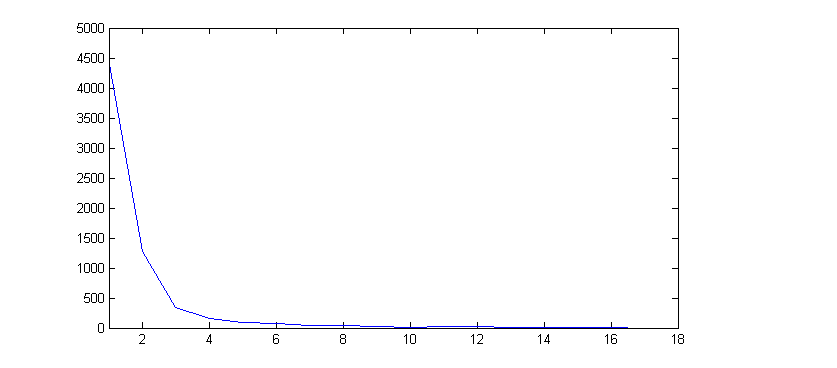
\includegraphics[scale=0.6]{figures/nbMoved.png} 
\caption{Number of moved objects per iteration during a typical clustering of 5000 objects.}
\end{figure}

\subsection{Memory access}

The lowered computational costs is also accompanied by a diminution in memory access: as can be seen from Equation~\ref{eq:newSimilNewC}, in order to compute the new object-to-class similarities after moving an object $n$, only line $n$ of the similarity matrix needs to be read. For the rest of the algorithm, only the (much smaller) object-to-class similarity matrix is used. By contrast, in the case of kernel k-means, the computation of $M_c$ values at each iteration require that the whole similarity matrix be read, which can be a serious performance bottleneck in the case of large object collections.

Moreover, the similarity update function of k-averages, by reading one line of the matrix at a time, presents good data locality properties, which make it play well with standard memory paging strategies.

To illustrate and confirm the theoretical complexity computed here, the next section proposes some performance figures measured on controlled datasets.


%\section{Comparison of approaches}
%
%(copy-pasted from the end of the former kkmeans section)
%
%
%However, it should be noted that this is an indirect result of a squared distance minimization objective, and that the impact of the third term of Eq~\ref{eq:yki} on the the minimized value is hard to quantify. This raises question as to the actual semantics of algorithms based on that objective function, and concerning the exact connection between the initial intent (similarity-based clustering) an the obtained result.
%
%Moreover, if a Euclidean geometric interpretation of the studied objects is not trivial\cad{}which is likely to be the case, otherwise the use of a simple k-means could be considered\cad{}then similarity values gathered into a matrix may not necessarily make a positive semi definite matrix, and thus not a proper kernel. To solve that problem, (Dhillon-Kulis) suggest, following (Roth-Laub), to offset all diagonal elements of the matrix by a constant value. Since directly computing the necessary offset to make the matrix positive definite is not feasible for such large matrices, the proposed solution consists in iteratively increasing the diagonal offset until the matrix tests positive. It appears clearly in Equation~ref{eq:yki} that this only adds a constant factor to the minimized objective function, and thus doesn't affect the optimal solution; however, as acknowledged by (Dhillon-Kulis), by affecting the spread of points and the weight distribution in the matrix, it does affect the operation of algorithms looking for that optimum in unforeseeable ways. \ml{too strong, for a well known problem, this impact can be studied in terms of convergence and quality of the solution and may be positive, so I guess that this unpredictability is only for new type of datasets.} \mr { toy example : point d'exclamation avec origin au bout du trait }
%
%Such is the price to pay to benefit from the solid geometric foundations and convergence guarantee of the k-means algorithm: a dissociation from immediate semantics, possibly made worse by the necessity of a clunky matrix conditioning procedure.
%
%Our purpose with the work presented in this paper is to propose an alternative algorithm that operates in a way very similar to kernel k-means, but is explicitly designed to process similarities, remains as close as possible to their semantics, and directly attempts to maximize a meaningful quantity: the average intra-class similarity.

\section{Validation}
\label{sec:validation}

In order to reliably compare the clustering quality and execution speed between the two approaches, we have written simple C implementations of Algorithms~\ref{algo:kkmeans_optim} and~\ref{algo:kaverages}, with minimal operational overhead: both read the similarity matrix from a binary file where all matrix values are stored sequentially in standard reading order, line by line, and write out the result of the clustering as a label text file. Both implementations use reasonably efficient code, but without advanced optimizations or parallel processing. All code can be found at <online reference>.

The figures presented in this section were obtained on simple synthetic datasets, in order to give precise control on the features of the analyzed data: for $n$ points split between $C$ classes, $C$ centroids are generated at random in 2D space, each point is given a random class, and point coordinates are generated following a Gaussian distribution around class centroids. In addition to numbers of objects and classes, the variance of Gaussian distributions can be adjusted to modulate how clearly separable clusters are. Similarities are computed as inverse Euclidean distances between points. This clearly simplified example is useful as a first control test bench; please refer to the next section for experiments on more realistic datasets.

\subsection{Clustering performance}

\begin{figure}
\label{fig:synth_perf}
\center
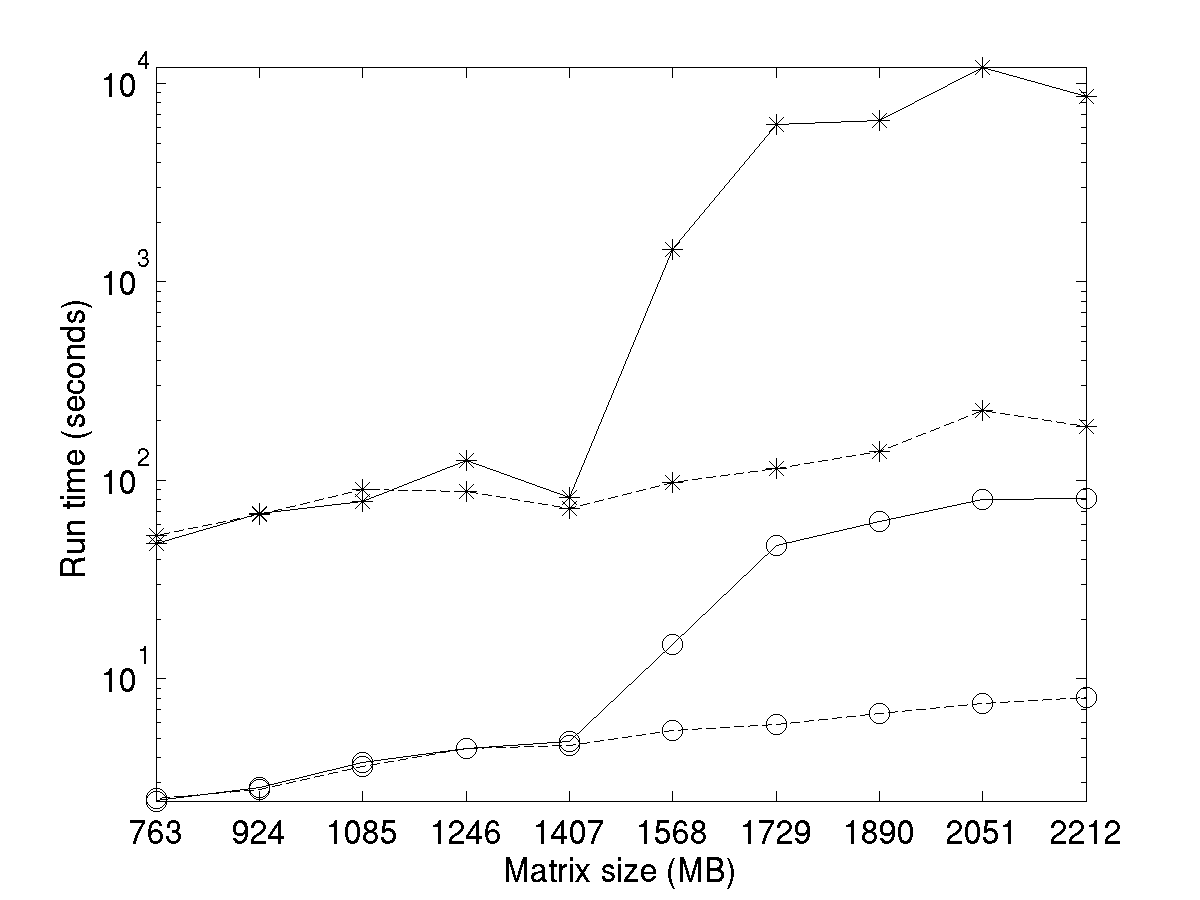
\includegraphics[scale=0.6]{figures/simpleSwap.png} 
\caption{MISSING FIGURE. NMI of kernel k-means and k-averages clustering relative to ground truth for synthetic data sets of varying sizes and \gl{difficulty} (degree of overlap between classes).}
\end{figure}

\subsection{Time efficiency}

Figure~\ref{fig:timing} shows the average time spent by kernel k-means and k-averages to cluster synthetic datasets or varying sizes. As previously, initial conditions on each run are identical for both algorithms.

\begin{figure}
\label{fig:timing}
\center
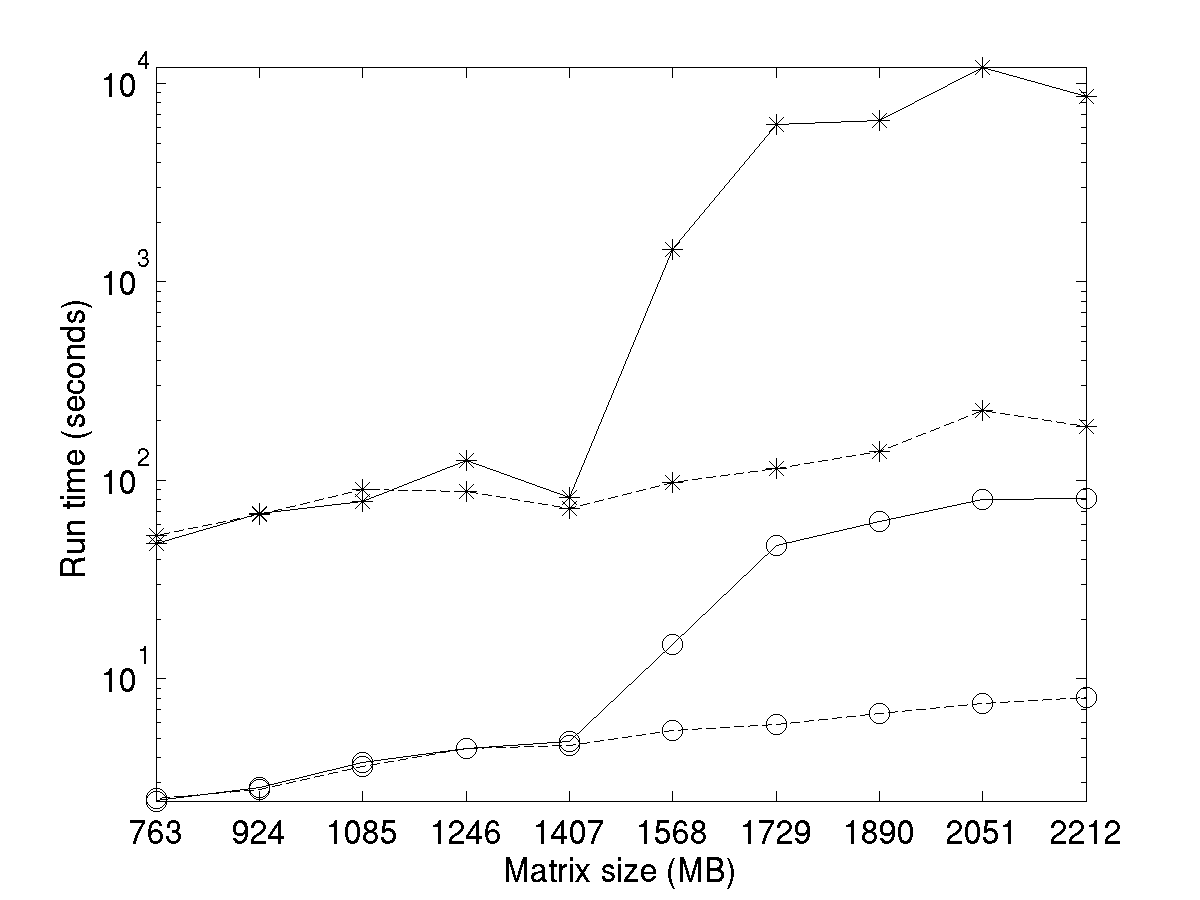
\includegraphics[scale=0.6]{figures/simpleSwap.png} 
\caption{Average computation time of the kernel k-means (*) and kaverages (o) algorithms on computers with 2 GB (solid line) and 32 GB (dashed line) of RAM, respectively. The \gl{running time} axis follows a logarithmic scale.}
\end{figure}

As can be seen, k-averages runs at least 20 times faster on average than kernel k-means in ordinary conditions, when  available memory is not an issue. When the matrix size exceeds what can be stored in RAM and the system has to resort to paged memory, as in the presented experiments when the matrix reaches about 1500MB, both algorithms suffer from a clear performance hit; however, kernel k-means is much more affected, and the difference becomes even more significant: with a 2000MB similarity matrix on a memory-limited computer, k-averages runs about 100 times faster than kernel k-means.


\section{Experiments}
\label{sec:experiments}

The previous section has established the satisfying behaviour of k-averages when running on synthetic test data; we now demonstrate its usefulness for real-life data, with the clustering of times series being selected as the evaluation task.

Time series, even though represented as vectors and therefore suitable for any kinds of norm-based clustering, are best compared with elastic measures (\cite{Ding:2008:QMT:1454159.1454226, Wang:2013:ECR:2429736.2429754}), due to their varying length. The Dynamic Time Warping (DTW) measure is an elastic measure widely used in many areas since its introduction for spoken word detection \cite{1163055} and has never been significantly challenged for time series mining (\cite{conf/kdd/BerndtC94, Rakthanmanon:2013:ABD:2513092.2500489}).

Effective clustering of time series using the DTW measure require similarity based algorithms such as the k-average algorithm. With some care, kernel based algorithm can also be considered provided that the resulting similarity matrix is converted into a kernel, \textit{i.e.} the matrix is forced to be semi definite positive to be a Gram matrix (\cite{Lanckriet:2004:LKM:1005332.1005334}).

\subsection{Datasets}

To compare the proposed algorithm to kernel k-means, a large collection of 43 time series datasets created by many laboratories all over the world and compiled by Prof. Keogh (\url{www.cs.ucr.edu/~eamonn/time_series_data}) is considered.  Statistics about the morphology of those datasets are summarized by Table \ref{tab:dbs}.

\begin{table}
\center
\begin{tabular}{l|ccc}
& min & average $\pm$ variance & max \\
\hline
number of classes & 2 & 8 $\pm$ 9 & 50 \\
number of time series & 56 & 1626 $\pm$ 2023 & 9236 \\
time series length & 24 & 372 $\pm$ 400 & 1882 \\
\end{tabular}
\caption{\label{tab:dbs} Statistics of the datasets. The length of the times series is expressed in samples.}
\end{table}


In order to ease comparison, the properties and the performance of clustering algorithms under evaluation are broken into 3 tables. Table \ref{tab:2} lists the bi-class datasets, \textit{i.e.} the datasets annotated in terms of presence or absence of a given property. Table \ref{tab:37} lists the datasets with a small number of classes (from 2 to 7) and Table \ref{tab:8} lists the datasets with a larger number of classes (from 8 to 50). 

\subsection{Evaluation Protocol}

For each dataset, since we perform clustering, and not supervised learning, the training and testing data are joined. If relevant, the DTW is computed using the implementation provided by Prof. Ellis (\url{http://www.ee.columbia.edu/~dpwe/resources/matlab/dtw}) with default parameters.

Clustering is done by requesting a number of clusters equal to the actual number of classes in the dataset. Clustering is repeated 20 times with varying initial conditions, \textit{i.e.} the initial assignment of points to clusters is randomly determined. For fairness of comparison, each algorithm is run with the exact same initial assignments.

Several metrics are available to evaluate the performance of a clustering algorithm. The one closest to the actual target application is the raw accuracy, that is the average number of items  labelled
correctly after an alignment phase of the estimated labelling of the reference one (\cite{Kuhn1955Hungarian}).

Another metric of choice, is the Normalized Mutual Information (NMI) criterion. Based on information theoretic principles, it measures the amount of statistical information shared by the random variables representing the predicted cluster distribution and the reference class distribution of the data points. If $P$ is the random variable denoting the cluster assignments of the points, and $C$ is the random variable denoting the underlying class labels on the points then the NMI measure is defined as:
\begin{equation}
\textbf{•}{NMI} = \frac{ 2\- I(C;K) }{H(C)+H(K)}
\end{equation}

where $I(X;Y)=H(X)−H(X|Y)$ is the mutual information between the random variables $X$ and $Y$, $H(X)$ is the Shannon entropy of $X$,and $H(X|Y)$ is the conditional entropy of $X$ given $Y$. Thanks to the normalization, the metric stays between $0$ and $1$, $1$ indicating a perfect match, and can be used to compare clustering with different numbers of clusters. Interestingly, random prediction gives an NMI close to $0$, whereas the accuracy of a random prediction on a balanced bi-class problem is 50\%.

For those reasons and ease of reading, only the NMI is considered here, as in (\cite{Kulis2008}). However, it shall be noted that most of the statements that will be made in the following in terms of ranking of the different algorithms  still holds true while considering the accuracy metric as reference, see \url{} for full results.

\subsection{Results}

  
\begin{table} 
\begin{center} 
\small 
 \setlength{\tabcolsep}{.16667em} 
\begin{tabular}{lllccccccccc} 
 &  &  &  &  &  & kMeans & kkMeans & kAverages & kAverages & kAverages & kAverages \\ 
\hline 
 &  &  &  &  &  &  &  & object & raw & object & raw \\ 
 &  &  & id & nbClasses & nbSamplesPerClass &  &  & p & p & b & b \\ 
 &  &  &  7 & 2 &      28$\pm$1 & 48$\pm$12 & \textbf{48$\pm$32} & \textbf{54$\pm$26} & \textbf{\textcolor{red}{66$\pm$32}} & \textbf{48$\pm$26} & \textbf{51$\pm$37} \\ 
 &  &  & 12 & 2 &    100$\pm$47 & 12$\pm$2 & 14$\pm$3 & \textbf{\textcolor{red}{15$\pm$0}} & 10$\pm$5 & \textbf{\textcolor{red}{15$\pm$0}} & 10$\pm$5 \\ 
 &  &  & 13 & 2 &     442$\pm$0 &  0$\pm$0 &  2$\pm$2 & \textbf{ 4$\pm$6} & \textbf{ 5$\pm$2} & \textbf{\textcolor{red}{9$\pm$12}} & \textbf{ 5$\pm$2} \\ 
 &  &  & 17 & 2 &     100$\pm$0 & 0 & 0 & 0 & \textbf{1} & 0 & \textbf{\textcolor{red}{1}} \\ 
 &  &  & 20 & 2 &     548$\pm$1 & \textbf{0$\pm$0} & \textbf{1$\pm$0} & \textbf{0$\pm$0} & \textbf{1$\pm$0} & \textbf{\textcolor{red}{1$\pm$5}} & \textbf{1$\pm$0} \\ 
 &  &  & 21 & 2 &     60$\pm$18 & \textbf{3$\pm$0} & 1$\pm$0 & 1$\pm$0 & \textbf{3$\pm$4} & 1$\pm$0 & \textbf{\textcolor{red}{4$\pm$4}} \\ 
 &  &  & 25 & 2 &    636$\pm$69 & 30$\pm$0 & \textbf{\textcolor{red}{52$\pm$0}} & 41$\pm$0 & 36$\pm$1 & 41$\pm$0 & 36$\pm$1 \\ 
 &  &  & 28 & 2 &    310$\pm$54 & 55$\pm$21 & \textbf{\textcolor{red}{ 78$\pm$0}} &  72$\pm$1 &  21$\pm$0 &  72$\pm$1 &  21$\pm$0 \\ 
 &  &  & 29 & 2 &   490$\pm$161 & \textbf{\textcolor{red}{24}} & 21 & 22 & 15 & 22 & 15 \\ 
 &  &  & 34 & 2 &     581$\pm$0 & 0$\pm$0 & 7$\pm$0 & 7$\pm$0 & \textbf{\textcolor{red}{8$\pm$0}} & 7$\pm$0 & \textbf{\textcolor{red}{8$\pm$0}} \\ 
 &  &  & 42 & 2 & 3582$\pm$3988 & \textbf{\textcolor{red}{0}} & 0 & 0 & 0 & 0 & 0 \\ 
 &  &  & 43 & 2 &  1650$\pm$170 & 0$\pm$0 & \textbf{\textcolor{red}{0$\pm$0}} & \textbf{0$\pm$0} & 0$\pm$0 & \textbf{0$\pm$0} & 0$\pm$0 \\ 
\end{tabular} 
\end{center} 
\caption{nbIterations: 200, distance: dtw, normalizeData: 1, nbRuns: 20} 
\label{nbit200DidtNoda1Nbru20} 
\end{table} 
 

  
\begin{table} 
\begin{center} 
\small 
 \setlength{\tabcolsep}{.16667em} 
\begin{tabular}{lllccccccccc} 
 &  &  &  &  &  & kMeans & kkMeans & kAverages & kAverages & kAverages & kAverages \\ 
\hline 
 &  &  &  &  &  &  &  & object & raw & object & raw \\ 
 &  &  & id & nbClasses & nbSamplesPerClass &  &  & p & p & b & b \\ 
 &  &  &  3 & 5 &      12$\pm$0 & \textbf{30$\pm$4} & 29$\pm$3 & \textbf{\textcolor{red}{32$\pm$2}} & \textbf{31$\pm$4} & 29$\pm$8 & 20$\pm$4 \\ 
 &  &  &  4 & 3 &     310$\pm$0 &  36$\pm$1 & \textbf{ 51$\pm$4} & \textbf{ 51$\pm$3} & 42$\pm$12 & \textbf{\textcolor{red}{ 52$\pm$3}} & 44$\pm$12 \\ 
 &  &  &  5 & 3 &  1436$\pm$755 & 0$\pm$0 & 0$\pm$0 & 0$\pm$0 & \textbf{0$\pm$0} & 0$\pm$0 & \textbf{\textcolor{red}{1$\pm$1}} \\ 
 &  &  &  6 & 4 &     355$\pm$0 & 23$\pm$3 & \textbf{44$\pm$8} & 41$\pm$5 & \textbf{\textcolor{red}{46$\pm$0}} & 40$\pm$7 & \textbf{45$\pm$4} \\ 
 &  &  & 11 & 4 &     80$\pm$31 & \textbf{\textcolor{red}{ 83$\pm$3}} & \textbf{81$\pm$10} & 65$\pm$10 & 57$\pm$16 & 21$\pm$20 & 32$\pm$27 \\ 
 &  &  & 15 & 4 &      28$\pm$5 &  45$\pm$4 &  67$\pm$9 & \textbf{72$\pm$10} &  63$\pm$3 & \textbf{\textcolor{red}{ 73$\pm$7}} &  65$\pm$7 \\ 
 &  &  & 18 & 5 &      93$\pm$9 &  9$\pm$0 & \textbf{ 9$\pm$1} & \textbf{\textcolor{red}{10$\pm$1}} &  8$\pm$1 & \textbf{ 9$\pm$2} &  8$\pm$1 \\ 
 &  &  & 19 & 7 &     93$\pm$22 & \textbf{5$\pm$1} & \textbf{5$\pm$1} & \textbf{5$\pm$0} & \textbf{\textcolor{red}{5$\pm$1}} & \textbf{5$\pm$0} & 5$\pm$1 \\ 
 &  &  & 22 & 7 &      20$\pm$8 &  44$\pm$2 &  51$\pm$4 &  50$\pm$2 & \textbf{\textcolor{red}{ 54$\pm$1}} & 44$\pm$15 & 37$\pm$15 \\ 
 &  &  & 26 & 6 &     74$\pm$20 & 22$\pm$3 & 23$\pm$3 & \textbf{\textcolor{red}{25$\pm$2}} & 21$\pm$1 & \textbf{24$\pm$2} & 21$\pm$2 \\ 
 &  &  & 27 & 4 &      15$\pm$8 &  66$\pm$4 &  59$\pm$9 &  61$\pm$7 & \textbf{\textcolor{red}{ 72$\pm$3}} & 53$\pm$19 & \textbf{70$\pm$11} \\ 
 &  &  & 30 & 3 & 3079$\pm$2045 & \textbf{60$\pm$0} & \textbf{\textcolor{red}{61$\pm$4}} & \textbf{60$\pm$0} & \textbf{61$\pm$0} & \textbf{60$\pm$0} & \textbf{61$\pm$0} \\ 
 &  &  & 32 & 6 &     170$\pm$9 &  76$\pm$6 & \textbf{ 79$\pm$4} & \textbf{\textcolor{red}{ 80$\pm$1}} &  77$\pm$5 & \textbf{77$\pm$18} & 68$\pm$17 \\ 
 &  &  & 33 & 4 &      50$\pm$0 &  53$\pm$2 & \textbf{\textcolor{red}{ 58$\pm$7}} &  53$\pm$3 &  52$\pm$2 & \textbf{ 56$\pm$6} & 43$\pm$15 \\ 
 &  &  & 35 & 4 &   1250$\pm$43 &   2$\pm$0 & \textbf{15$\pm$13} &  11$\pm$8 & \textbf{12$\pm$13} & \textbf{\textcolor{red}{ 16$\pm$7}} & \textbf{13$\pm$12} \\ 
 &  &  & 37 & 7 &      50$\pm$0 &  31$\pm$2 & \textbf{ 42$\pm$2} & \textbf{\textcolor{red}{ 42$\pm$2}} &  40$\pm$2 & \textbf{38$\pm$10} &  17$\pm$8 \\ 
 &  &  & 38 & 6 &     100$\pm$0 &  79$\pm$3 &  84$\pm$4 & \textbf{ 87$\pm$5} & \textbf{\textcolor{red}{ 87$\pm$1}} &  84$\pm$5 & 65$\pm$26 \\ 
\end{tabular} 
\end{center} 
\caption{nbIterations: 200, distance: dtw, normalizeData: 1, nbRuns: 20} 
\label{nbit200DidtNoda1Nbru20} 
\end{table} 
 

  
\begin{table} 
\begin{center} 
\small 
 \setlength{\tabcolsep}{.16667em} 
\begin{tabular}{lllccccccccc} 
 &  &  &  &  &  & kMeans & kkMeans & kAverages & kAverages & kAverages & kAverages \\ 
\hline 
 &  &  &  &  &  &  &  & object & raw & object & raw \\ 
 &  &  & id & nbClasses & nbSamplesPerClass &  &  & p & p & b & b \\ 
 &  &  &  1 & 50 &   18$\pm$21 &  64$\pm$1 &  70$\pm$1 &  71$\pm$1 & \textbf{\textcolor{red}{ 72$\pm$1}} & 26$\pm$29 &  12$\pm$0 \\ 
 &  &  &  2 & 37 &    21$\pm$2 &  58$\pm$1 & \textbf{\textcolor{red}{ 62$\pm$1}} &  60$\pm$1 &  58$\pm$1 & 26$\pm$25 &  10$\pm$1 \\ 
 &  &  &  8 & 12 &    65$\pm$0 & 26$\pm$1 & 29$\pm$2 & \textbf{\textcolor{red}{31$\pm$1}} & 27$\pm$2 & \textbf{29$\pm$7} & 19$\pm$9 \\ 
 &  &  &  9 & 12 &    65$\pm$0 & 30$\pm$1 & \textbf{35$\pm$2} & \textbf{35$\pm$1} & 33$\pm$1 & \textbf{\textcolor{red}{35$\pm$1}} & 24$\pm$9 \\ 
 &  &  & 10 & 12 &    65$\pm$0 & 25$\pm$1 & 30$\pm$1 & \textbf{\textcolor{red}{31$\pm$1}} & 28$\pm$2 & \textbf{30$\pm$7} & 20$\pm$9 \\ 
 &  &  & 14 & 14 &  161$\pm$73 &  37$\pm$2 & \textbf{\textcolor{red}{ 77$\pm$3}} &  74$\pm$1 &  67$\pm$3 &  74$\pm$2 & 57$\pm$17 \\ 
 &  &  & 16 & 14 &  161$\pm$73 &  37$\pm$2 & \textbf{ 77$\pm$3} & \textbf{\textcolor{red}{ 77$\pm$2}} &  70$\pm$3 & \textbf{72$\pm$17} & 52$\pm$21 \\ 
 &  &  & 23 &  8 &   300$\pm$0 &  87$\pm$5 & \textbf{ 88$\pm$5} &  87$\pm$3 & \textbf{\textcolor{red}{ 90$\pm$4}} & 75$\pm$33 & 45$\pm$26 \\ 
 &  &  & 24 & 10 & 114$\pm$171 & 25$\pm$1 & \textbf{\textcolor{red}{32$\pm$1}} & 30$\pm$2 & 31$\pm$2 & 28$\pm$7 & 25$\pm$8 \\ 
 &  &  & 31 & 15 &    75$\pm$0 &  54$\pm$2 & \textbf{ 66$\pm$3} & \textbf{\textcolor{red}{ 67$\pm$2}} &  56$\pm$2 & 40$\pm$33 & 10$\pm$12 \\ 
 &  &  & 36 & 25 &   36$\pm$41 &  42$\pm$1 & \textbf{ 51$\pm$1} & \textbf{\textcolor{red}{ 51$\pm$1}} &  51$\pm$1 & 30$\pm$25 & 16$\pm$16 \\ 
 &  &  & 39 &  8 &   560$\pm$0 & 44$\pm$1 & \textbf{46$\pm$1} & \textbf{\textcolor{red}{46$\pm$0}} & \textbf{46$\pm$1} & \textbf{46$\pm$1} & \textbf{45$\pm$5} \\ 
 &  &  & 40 &  8 &   560$\pm$0 & 44$\pm$0 & \textbf{45$\pm$0} & 44$\pm$0 & \textbf{\textcolor{red}{45$\pm$1}} & 44$\pm$0 & \textbf{44$\pm$5} \\ 
 &  &  & 41 &  8 &   560$\pm$0 &  0$\pm$0 & 43$\pm$1 & \textbf{44$\pm$1} & 42$\pm$1 & \textbf{\textcolor{red}{44$\pm$0}} & 42$\pm$0 \\ 
\end{tabular} 
\end{center} 
\caption{nbIterations: 200, distance: dtw, normalizeData: 1, nbRuns: 20} 
\label{nbit200DidtNoda1Nbru20} 
\end{table} 
 


\subsection{From Progressive to Batch Updates}

\subsection{From Raw to Object Normalized Criterion}


\section{Discussion}

\section{Conclusion}

\bibliography{bib}

\appendix

  
\begin{table} 
\begin{center} 
\ 
 \setlength{\tabcolsep}{.16667em} 
\begin{tabular}{lc} 
dataSet & id \\ 
\hline 
50words &  1 \\ 
Adiac &  2 \\ 
Beef &  3 \\ 
CBF &  4 \\ 
ChlorineConcentration &  5 \\ 
CinC\_ECG\_torso &  6 \\ 
Coffee &  7 \\ 
Cricket\_X &  8 \\ 
Cricket\_Y &  9 \\ 
Cricket\_Z & 10 \\ 
DiatomSizeReduction & 11 \\ 
ECG200 & 12 \\ 
ECGFiveDays & 13 \\ 
FaceAll & 14 \\ 
FaceFour & 15 \\ 
FacesUCR & 16 \\ 
Gun\_Point & 17 \\ 
Haptics & 18 \\ 
InlineSkate & 19 \\ 
ItalyPowerDemand & 20 \\ 
Lighting2 & 21 \\ 
Lighting7 & 22 \\ 
MALLAT & 23 \\ 
MedicalImages & 24 \\ 
MoteStrain & 25 \\ 
OSULeaf & 26 \\ 
OliveOil & 27 \\ 
SonyAIBORobotSurface & 28 \\ 
SonyAIBORobotSurfaceII & 29 \\ 
StarLightCurves & 30 \\ 
SwedishLeaf & 31 \\ 
Symbols & 32 \\ 
Trace & 33 \\ 
TwoLeadECG & 34 \\ 
Two\_Patterns & 35 \\ 
WordsSynonyms & 36 \\ 
fish & 37 \\ 
synthetic\_control & 38 \\ 
uWaveGestureLibrary\_X & 39 \\ 
uWaveGestureLibrary\_Y & 40 \\ 
uWaveGestureLibrary\_Z & 41 \\ 
wafer & 42 \\ 
yoga & 43 \\ 
\end{tabular} 
\end{center} 
\caption{normalizeData: 1} 
\label{noda1} 
\end{table} 
 


\end{document}
